\documentclass{article}

% Required packages (merged from hw5_template.tex and hw6_questions.tex)
\usepackage{amssymb}
\usepackage{amsmath}
\usepackage{graphicx}
\usepackage{geometry}
\usepackage{tikz}
\usepackage{array}
\usepackage{booktabs}
\usepackage{enumitem}
\usepackage{listings}
\usepackage{xcolor}
\usepackage{fancyhdr}
\usepackage{float}
\usepackage{subcaption}
\usepackage{comment}
\usepackage{algorithm}
\usepackage{algpseudocode}
\usepackage{caption}
\usepackage{siunitx}
\usepackage{hyperref}
\usetikzlibrary{arrows.meta, positioning} % Required for hw6 diagrams

% Set page geometry
\geometry{a4paper, margin=1in}

% Configure listings for Python
\lstset{
  language=Python,
  basicstyle=\ttfamily\footnotesize,
  numbers=left,
  numberstyle=\tiny\color{gray},
  frame=single,
  breaklines=true,
  breakatwhitespace=true,
  captionpos=b,
  tabsize=4,
  showspaces=false,
  showstringspaces=false,
  showtabs=false,
  commentstyle=\color{gray}\textit,
  keywordstyle=\color{blue}\bfseries,
  stringstyle=\color{red}
}

\begin{document}

\pagestyle{fancy}
\lhead{DSC 257: Unsupervised Learning (Fall 2025)}
\rhead{Lecture Summary: HW 7}

%------------------
% Section 1: Markov Random Fields
%------------------
\section{Markov Random Fields}
\subsection{Markov Random Fields: Introduction}
\subsubsection{Disease Example}
\begin{flushleft}
    We are given the following:
    \begin{itemize}
        \item Four people (two female, two male) engage in occasional pairwise activities
        \item There is a disease going around
        \item Let Boolean random variables $F_1$,$F_2$,$M_1$,$M_2$ denote the disease status ($0|1$)
        \item Interaction graph $G$ is seen below:
    \end{itemize}
\end{flushleft}
\begin{figure}[h!]
\centering
%\begin{center}
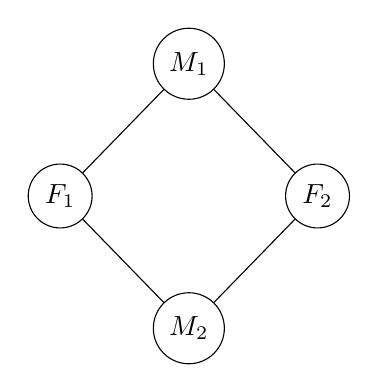
\begin{tikzpicture}[node distance=1cm]
\node[circle,draw] (W) {$M_1$};
\node[circle,draw,below=of W,color=white] (C) {$.$};
\node[circle,draw,below=of C] (Y) {$M_2$};
\node[circle,draw,right=of C] (X) {$F_2$};
\node[circle,draw,left=of C] (Z) {$F_1$};

\draw (W) -- (X);
\draw (X) -- (Y);
\draw (Y) -- (Z);
\draw (Z) -- (W);
\end{tikzpicture}
\caption{Interaction graph for disease example}
\label{fig:projection_x_on_u}
\end{figure}
\begin{flushleft}
    A distributuon $P(F_1,F_2,M_1,_M2)$ factors over graph $G$ if:
\end{flushleft}
$$
P(F_1,F_2,M_1,_M2) = \frac{1}{Z} \psi_{11}(F_1,M_1)\psi_{12}(F_1,M_2)\psi_{21}(F_2,M_1)\psi_{22}(F_2,M_2)
$$
\begin{flushleft}
    where:
    \begin{itemize}
        \item $\psi_{11}$,$\psi_{12}$,$\psi_{21}$,$\psi_{22}$ are arbitary positive-valed functions
        \item $Z$ is a normalizing factor
    \end{itemize}
\end{flushleft}
\begin{table}[h]
\centering
\begin{tabular}{llc}
\toprule
$F_1$ & $M_1$ & $\psi_{11}(F_1,M_1)$ \\
\midrule
0 & 0 & 100 \\
0 & 1 & 20 \\
1 & 0 & 20 \\
1 & 1 & 50 \\
\bottomrule
\end{tabular}
\quad
\begin{tabular}{llc}
\toprule
$F_1$ & $M_2$ & $\psi_{12}(F_1,M_2)$ \\
\midrule
0 & 0 & 100 \\
0 & 1 & 20 \\
1 & 0 & 20 \\
1 & 1 & 50 \\
\bottomrule
\end{tabular}

\vspace{0.25em}

\begin{tabular}{llc}
\toprule
$F_2$ & $M_1$ & $\psi_{21}(F_2,M_1)$ \\
\midrule
0 & 0 & 200 \\
0 & 1 & 10 \\
1 & 0 & 100 \\
1 & 1 & 50 \\
\bottomrule
\end{tabular}
\quad
\begin{tabular}{llc}
\toprule
$F_2$ & $M_2$ & $\psi_{22}(F_2,M_2)$ \\
\midrule
0 & 0 & 100 \\
0 & 1 & 20 \\
1 & 0 & 20 \\
1 & 1 & 1 \\
\bottomrule
\end{tabular}
\vspace{1em}
\caption[Psi Tables]{psi tables are seen above for each outcome}
\label{tab:psi_table}
\end{table}

\newpage

\begin{flushleft}
    \textit{What is the normalizing factor $Z$}
\end{flushleft}

\noindent\rule{\textwidth}{0.4pt}\\

\subsubsection*{Find Normalizing Factor $Z$}

\subsubsection*{\normalfont}{$\therefore$ }

\noindent\rule{\textwidth}{0.4pt}\\

\begin{flushleft}
    From \textit{Table 1} we can construct the following table:
\end{flushleft}

\begin{table}[h]
\centering
\begin{tabular}{cccc|c}
\toprule
$F_1$ & $F_2$ & $M_1$ & $M_2$ & $\psi_{11}(F_1,M_1)\psi_{12}(F_1,M_2)\psi_{21}(F_2,M_1)\psi_{22}(F_2,M_2)$ \\
\midrule
0 & 0 & 0 & 0 & $100\times100\times200\times100$ \\
0 & 0 & 0 & 1 & $100\times20\times200\times20$ \\
0 & 0 & 1 & 0 & $20\times100\times10\times100$ \\
0 & 0 & 1 & 1 & $20\times20\times10\times20$ \\
0 & 1 & 0 & 0 & $100\times100\times100\times20$ \\
0 & 1 & 0 & 1 & $100\times20\times100\times1$ \\
0 & 1 & 1 & 0 & $20\times100\times50\times20$ \\
0 & 1 & 1 & 1 & $20\times20\times50\times1$ \\
1 & 0 & 0 & 0 & $20\times20\times200\times100$ \\
0 & 0 & 0 & 1 & $20\times50\times200\times20$ \\
1 & 0 & 1 & 0 & $50\times20\times10\times100$ \\
1 & 0 & 1 & 1 & $50\times50\times10\times20$ \\
1 & 1 & 0 & 0 & $20\times20\times100\times20$ \\
1 & 1 & 0 & 1 & $20\times50\times100\times1$ \\
1 & 1 & 1 & 0 & $50\times20\times50\times20$ \\
1 & 1 & 1 & 1 & $50\times50\times50\times1$ \\
\bottomrule
\end{tabular}

\vspace{1em}
\caption[Most likely Table]{most likely table}
\label{tab:cfg_table}
\end{table}

\begin{flushleft}
    \textit{What is the most likely configuration?}
\end{flushleft}

\noindent\rule{\textwidth}{0.4pt}\\

\subsubsection*{Find Most Likely Configuration}

\subsubsection*{\normalfont}{$\therefore$ }

\noindent\rule{\textwidth}{0.4pt}\\

\subsubsection{Clique Potentials}
\begin{flushleft}
    Given a joint distribution over random variables $X_1$,...,$X_n$ such that:
    \begin{enumerate}
        \item An undirected graph with nodes $X_1$,...,$X_n$ and edges representing dependencies
        \item A distribution that factors over this graph:
    \end{enumerate}
    $$
    P(X_1,...,X_n) = \frac{1}{Z} \prod_{C} \psi_C (\{ X_i:i\in C\})
    $$
    where the product is over maximal cliques in the graph, and the clique potentials $\psi_C$ are positive-valued functions
\end{flushleft}

\subsubsection*{Example}
\begin{flushleft}
    Given the Interaction graph:
\end{flushleft}
\begin{figure}[h!]
\centering
%\begin{center}
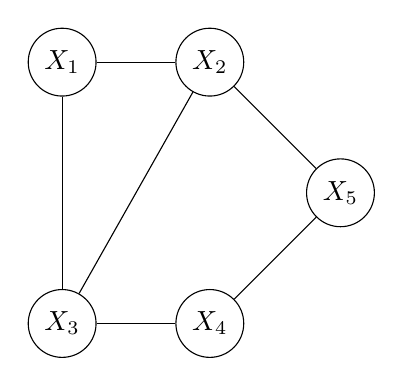
\begin{tikzpicture}[node distance=1cm]
\node[circle,draw] (W) {$X_2$};
\node[circle,draw,below=of W,color=white] (C) {$.$};
\node[circle,draw,below=of C] (Y) {$X_4$};
\node[circle,draw,left=of Y] (X) {$X_3$};
\node[circle,draw,left=of W] (A) {$X_1$};
\node[circle,draw,right=of C] (Z) {$X_5$};

\draw (W) -- (Z);
\draw (W) -- (X);
\draw (Y) -- (Z);
\draw (X) -- (Y);
\draw (A) -- (X);
\draw (A) -- (W);
\end{tikzpicture}
\caption{Interaction graph for clique potential example}
\label{fig:clique_ex}
\end{figure}
\begin{flushleft}
    The functional form of $P(X_1,X_2,X_3,X_4,X_5)$ is: 
\end{flushleft}
$$
\frac{1}{Z}\psi_{123}(X_1,X_2,X_3)\psi_{25}(X_2,X_5)\psi_{34}(X_3,X_4)\psi_{45}(X_4,X_5)
$$

\subsubsection*{Lecture Transcript}
\begin{flushleft}
    So in this second part of the course, our theme has been modeling data using probability distributions, that is fitting distributions to data. We began with the simplest distributions for one dimensional data, distributions like the Gaussian and the Poisson. Then we moved on to higher dimensional data where we began with the multi-variate Gaussian. Most recently we've looked at Bayes' nets, which use directed graphs to represent distributions of arbitrary complexity. Bayes' nets are sometimes called directed graphical models. We'll now turn to undirected graphical models, which are more commonly known as Markov random fields. So as usual, let's begin with an example from the classic textbook by Judea Pearl. In this example, there are four people, two men and two women, and these people occasionally meet in pairs, one man and one woman. There's also a disease going around. So for each of the people we define a binary random variable that represents whether or not they have the disease. So we have four random variables, F1 and F2 for the women, and M1 and M2 for the men. And each of these takes on value zero or one, no disease or disease. We are interested in modeling the joint distribution over these four random variables. Now on the right over here we have a graph that captures the interactions between the people. So the first man, for example, occasionally meets with the first woman, and occasionally meets with the second woman. So this is an interaction graph, but in this case the dependencies between the random variables arise solely from these interactions. So this is also a dependency graph. Now, what we are interested in is the joint distribution over these four random variables. This could be anything, but we say that the joint distribution factors over this graph, if it has this functional form, if the joint distribution can be written in this way. Let's see what this is saying. What it's saying is that the probability of any configuration, F1, F2, M1, M2 is the product of four terms. The first term only involves F1 and M1. It only involves these two variables. The second term only involves F1 and M2. The third term only involves F2 and M1, and the fourth term only involves F2 and M2. Now, each of these terms is a function just of that pair of random variables. So we are gonna call them Psi11, Psi12, Psi21, Psi22. And these are arbitrary functions. The only thing that we require is that these functions have positive values. Other than that, they could be anything. Now, in order for this to be a valid probability distribution, we do need the probabilities of all the configurations to add up to one, and because of that, we have this normalizing factor in the front, okay? So the only purpose of that is to make sure that everything adds up to one. So what this functional form is saying is that the distribution does not have arbitrary dependencies. In fact, the probability of any configuration, F1, F2, M1, M2 can be obtained just by looking at pairs of random variables, the pairs that interact. There are no dependencies beyond this. So that sounds intuitive, but what are these functions exactly? What are these Psi11, Psi12, and so on? Let's look at an example. So here's an example of what these functions might be. So we have four functions. One for F1 M1, and functions for each of the other edges as well. So let's focus on this particular function, Psi11. It's a function of F1 and M1, and F1 and M1 are both binary. So they each take on value zero and one, which means that the function can be specified with a little table like this. A table that simply enumerates the four possible configurations of the inputs F1 and M1. And for each of those configurations it gives the function value. Now, notice that these function values don't add up to one, or anything like that. They're pretty arbitrary numbers. The important thing is just that they are positive, okay, so that's the first function, what we call the first clique potential. Likewise, the other functions might look like this. Each of them can be captured by a small table. Now, what is the probability of a particular configuration? So let's say that we are interested in a configuration like this, the probability that, let's say, everybody has the disease except the second man. So the probability that they're all one except for M2, which is zero. What is the probability of that? Well, we'll just plug into this formula. It's one over the normalizing factor, times Psi11 of F1, M1. So that's this entry over here. So 50 times Psi12 of F1, M2. So that's this entry over here, 20. Psi21 of F2, M1. So that's this entry over here, (clicking) and Psi22 of F2, M2, which is this entry over here. That's the probability of that particular configuration. Now, notice that in order to get a concrete probability we really need this normalizing factor. We need to know what it is. What is it? So here I've made a large table, containing all possible configurations of the four random variables. Since they're Boolean, since they each take on just two possible values, the total number of possible configurations is two times two times two times two, which is 16, which isn't too much. And so I've just made a big table, and for each configuration, I've written down the product of the values of the four functions. The normalizing factor is the sum of these. (clicking) If we divide by this normalizing factor we get legitimate probabilities. Now, in this case the normalizing factor is not that hard to figure out because the total number of configurations is only 16. But in more general scenarios, where there are lots more random variables, or where the random variables take on more values, where they're not just binary, the number of configurations could be truly enormous, could be exponentially large. In such cases, it will be really hard to determine the normalizing factor, and that's a problem that we are gonna have to grapple with. But in the meantime, is there anything we can do without knowing the normalizing factor? It turns out there's actually plenty we can do without knowing Z. For example, we can figure out the most likely configuration. The most likely configuration is simply the largest number in this table, which is this one. It is the configuration where nobody has the disease. Okay. Now that we have looked at a brief example let's go back and define Markov random fields a little bit more formally. So Markov random fields are a way of representing a joint distribution over multiple random variables with the help of a graph. Hmm, that sounds a lot like Bayes' nets. Yes, but the difference is that now we use undirected graphs, rather than directed graphs. Let's say for example, that we have five random variables, and we want to capture the joint distribution over these variables. So the first thing we do is to draw a graph that captures interactions or dependencies between the variables. Once we have this graph, it immediately tells us the functional form of the distribution. It tells us that the distribution must look like this. Where do we get this from? Where is this functional form coming from? How do we go from the graph to this particular functional form? The way we do that is by looking at maximal cliques in the graph. Now, a clique is a collection of nodes that are fully connected that have all possible edges between them. So for example, the click, examples of cliques in this graph are X1, X2, and X3. (clicking) This is a clique because we have three nodes and all possible edges between them are present. Okay, what about X1, (clicking) X3, and X4? (clicking) Is that a click? No, it's not a click because there's no edge between X1 and X4. So this doesn't count as a click. Okay? So one of the cliques is X1, X2, and X3, and moreover, it's a maximal click. What that means is that we cannot add to it. There is no extra node we can add to that, while retaining the clique property. So that's one of the maximal cliques in the graph. What are the other maximal cliques? Well, X4 and X5, just by themselves. This pair are a maximal click. There's only one possible edge between them that edge is present, and there is nothing we can add to those two while still retaining the clique property. So that's another maximal click. As is X2, X5. (clicking) Okay, this edge. And X3, X4. (clicking) This edge. And in fact these are the only maximal cliques in the graph. This graph has four maximal cliques. Now, that tells us that the functional form of the distribution looks like this. (clicking) It is the product of four terms, one for each of the cliques. So there's a term for one, two, three, which only involves the variables in that click. There's a second function that only involves the variables in this click. Another function that only involves the variables in this click, and another function that only involves the variables in that click. Now, these functions can be completely arbitrary, except that they must be positive. And in order to get a legitimate probability distribution, we need this normalizing factor in the beginning to make sure that everything adds up to one. Now, this is just an example with five variables. More generally, we'll have a distribution over N variables. And in order to do that, we begin with an undirected graph with nodes for each of the variables and where the edges represent dependencies between variables. Once we have the graph, a distribution that factors over this graph is a distribution that has this functional form, where the probability of any configuration is given by a product of functions, one for each click. So let's see, be one of the cliques in the graph. So let's see, be a maximal clique in the graph. (clicking) There is a function for each such maximal click, and is it is a function of only the variables in that click. The function only looks at the nodes inside that click. We will sometimes use X sub c as a shorthand for these variables. X sub c is all variables Xi that lie inside that clique. Okay, so a distribution factors over the graph, if it can be expressed as a product of functions one for each maximal clique in the graph. These functions are called clique potentials. They're allowed to be arbitrary, except that they must be positive, and then we have a normalizing factor in the front. What this tells us is that the joint distribution over the end variables is not arbitrary. The dependencies between the variables are not arbitrary. The joint distribution is a product of local terms. Each term corresponds to a clique, a bunch of fully interacting random variables, and we can get the full probability of a configuration by just looking at these local terms, and multiplying them together. Okay? So that's the formalism of the Markov random field. Next time, we'll look more closely at some properties of these models. 
\end{flushleft}


%------------------
% Section 2: Markov Random Fields
%------------------
\subsection{Markov Random Fields: Conditional Independence Properties}
\subsubsection{Conditional Independence Example}
\begin{flushleft}
    Given: Alice and Bod don't know each other but drive home from work along the same road. Alice is late for dinner if she leaves work late, or if there is a lot of traffic that day; likewise with Bob.
\end{flushleft}

\begin{flushleft}
    Define the three boolean variables $A$,$B$,$T$ as:
    \begin{itemize}
        \item $A$: Is Alice late for dinner?
        \item $B$: is Bob late for dinner?
        \item $T$: Is there a lot of traffic that day?
    \end{itemize}
\end{flushleft}
\begin{flushleft}
    We have the following questions:
    \begin{enumerate}
        \item Is $A$ independent of $B$?
        \item Is $A$ independent of $B$ given $T$
    \end{enumerate}
\end{flushleft}
\begin{flushleft}
    Let, $X$,$Y$,$Z$ be random variables defined on the same space.
\end{flushleft}
\begin{flushleft}
    We say $X$ is conditionally independent of $Y$ given $Z$ if for all $x$,$y$,$z$:
\end{flushleft}
$$
Pr(X=x,Y=y|Z=z) = P(X=x|Z=z)P(Y=y|Z=z)
$$

\subsubsection{Local and Global Independence Property}
\begin{flushleft}
    Let $G$ be an undirected graph with nodes $X_1$,...,$X_n$ \\
    Let $N_G(X_i)$ denote the neighbors of $X_i \in G$\\
    Suppose the distribution $P(X_1,...,X_n)$ factors over this graph. Then it satfies the two following properties:
    \begin{enumerate}
        \item Local independence property: for any $i$,
        $$X_i \text{(idk symbol for independent)} \{X_j:j\neq i\}|N_G(X_i)$$
        \item Global independence property: for any subsets of nodes $S$,$T$,$U$ such that removing $U$ separtes $S$ from $T$,
        $$X_S \text{(idk symbol for independent)} X_T | X_U$$
    \end{enumerate} 
\end{flushleft}

\subsubsection{The Hammersley-Clifford Theorem}
\begin{flushleft}
    Let $P$ be a distribution on $(X_1,...,X_n)$ such that:
    \begin{itemize}
        \item $P(X)>0 for all $x$ and$
        \item $P$ satisfies the local independence properties
        \begin{itemize}
            \item Then $P$ is a Markov random field that factors over $G$
        \end{itemize}
    \end{itemize}
    Simple Translation: From the qualitative conditional independence properties of a distribution we can infer its precise functional form
\end{flushleft}

\subsubsection*{Lecture Transcript}
\begin{flushleft}
    So we have briefly introduced Markov random fields. Now, a key concept in understanding these models is conditional independence. So let's explore this a little bit. Let's start with a little example, a little toy example of conditional independence. So let's say we have two people, Alice and Bob, who don't know each other. They are complete strangers. However, every evening, they drive home from work along the same road. Now, Alice is late for dinner if one of two things happens. Either she leaves work late or there happens to be a lot of traffic that day along that road. Similarly with Bob, he's late for dinner if one of two things happens, either he leaves late, or there's a lot of traffic along that road. So let's define three Boolean random variables that pertain to this situation. The first variable, A, tells us whether Alice is late for dinner. It's A equals one if Alice is late, otherwise A equals zero. Variable B says whether Bob is late for dinner. And variable T says whether there's a lot of traffic that day. Three Boolean random variables. Now let's answer some questions. First of all, are A and B independent? No, they're not. If Alice is late for dinner, that means it's more likely that there's a lot of traffic that day, which means that it's also more likely that Bob is late for dinner. That's strange. So these two people are complete strangers, and yet whether they're late for dinner is not independent, okay? It is the traffic that binds them together. Now suppose we condition on the traffic. Is A independent of B given T? So for example, let's say that there is no traffic that day, T equals zero. Is A independent of B given that? And the answer is yes, because if there's no traffic, the only thing that can make Alice late is leaving late. And the only thing that can make Bob late is leaving late. And those two events are independent. So we'll say that A is independent of B conditioned on T equals zero. What if T equals one? What if there's a lot of traffic that day? Okay, so there's a lot of traffic. That means it's more likely that A is late, that Alice is late and that Bob is late. But still, whether they're actually late just depends on the additional information of whether they leave work late. So once again, A is independent of B given this information. And so we have two random variables, A and B, that are not independent, but they are independent conditioned on T. The way we draw this using a graphical model is something like this. We have three random variables and A and B are correlated. There is some dependence between them, but the only dependence between them is mediated through T. So A and B are not independent, but once you condition on T, it's like removing this node, and it breaks A and B apart, it makes them independent. Okay, so that was just a little example for some intuition. Now let's go ahead and formally define conditional independence. So we have three random variables, X, Y, and Z. And we say that X is conditionally independent of Y given Z if the following holds. If for all possible settings of these variables, little x, little y, and little z, the probability that X is little x and Y is little y given that Z is little z is equal to the probability that X is little x given Z is little z times the probability that Y is little y given that Z is little z. Okay, in other words, if we condition on the event that Z takes this value, X and Y behave like they're independent, so we write it like this. X is independent of Y given Z. That's the notation. Okay, so let's look at another example now. Let's say that X and Y are independent coin flips taking values zero and one, okay? So they're each zero or one with probability 1/2 and they're independent, and let Z be the and of X and Y, okay? So Z is one if both X and Y are one, otherwise Z is zero. Is X conditionally independent of Y given Z? Hmm. Well, let's see. First of all, we do know that X is independent of Y. We are told that. So good, we've got that. But now what happens when we condition on Z? Well, let's see, suppose we have Z equals zero. What does that tell us? It tells us that X and Y cannot both be one. In other words, if X is one, then Y has to be zero. That means that X and Y are not independent conditioned on Z equals zero. So X and Y are not independent conditioned on Z. So here we have a situation where X and Y are independent just by themselves, but when we introduce this third random variable Z, it creates a dependence between them. They stop being independent when we condition on Z. Okay, so now let's return to our example from last time, the example from Pearl's textbook in which there are four individuals, two men and two women, and there's a disease going around. Now, the interactions between these four people are captured by this interaction graph, this dependency graph, and in defining Markov random fields, we said that a distribution factors over this graph if it has this functional form, if the distribution, if the joint distribution of any set of four values, of any configuration can be expressed as a product of local terms, one for each of the edges in this graph. In other words, you can figure out the probability of any configuration just by looking at pairs of variables, pairs of people that interact. And for example, these are what these functions, which we call clique potentials, might be. Okay. The values of the functions are arbitrary. What matters is just that they're positive. Now, what are the conditional independence properties of such a distribution? So let's look at the two women, for example. Is F1 independent of F2? There's no edge between them, but they are dependent because they can communicate a disease from one to the other through either of the two men. So they are not independent of each other. However, they are conditionally independent given the status of the two men. And likewise, the two men are conditionally independent of each other, their disease status is conditionally independent of each other given the status of the two women. So these are the conditional independence properties of this distribution. Now, this seems fairly intuitive from the graph, but conditional independence is a mathematical property. So we should go ahead and try to establish this formally to see how we can arrive at this conclusion solely from this functional form. Okay, so this is what our distribution looks like. And what we wanna check is, for example, that M1 is independent of M2 given F1 and F2. How would we do this? Well, let's pick any values for F1 and F2. Remember, they're binary, so they're in the range zero or one. So pick any values, little f1 and little f2. And now let's see, the probability of M1 and M2 conditioned on F1 being little f1 and F2 being little f2. What is it? Well, we don't know what this normalizing factor is. Doesn't matter. It's proportional, okay? This is the proportional sign. It's proportional to these four functions, which is psi one, one times, now we plug in the specific value little f1. M1 is still a variable, okay? And now we plug in, again, the specific value little f1, while M2 is still a variable. And likewise, we get psi two, one with little f2 and the variable M1, and psi two, two with little f2 and the variable M2. So now let's reorganize these terms. Let us group together these two. So we get something like this. And then let's group together the other two. And so we get something like this. And so if you notice, over here, we have a function only of M1. And over here, we have a function of only M2. And so the probability of any pair M1, M2 conditioned on the values little f1 and little f2 are something that depends only on capital M1 times something that depends only on capital M2. So M1 and M2 are indeed independent conditioned on F1 and F2. So now that we've looked at this little example, let's move on to Markov random fields in greater generality. So let's start by recalling the definition of a Markov random field. So we have a joint distribution over n random variables, say X1 through Xn. And the way we specify this distribution is by first drawing an undirected graph with a node for each of these variables and where the edges capture dependencies between variables. Once we've specified the graph, we say that a joint distribution P factors over the graph, conforms to the graph if it happens to have the following functional form. If it can be expressed as the product of a bunch of local terms, where there is a local term for each maximal clique in the graph. And that local term is a function called a clique potential that depends only on the variables inside that clique. So a distribution factors over the graph if it can be expressed as the product of local terms, one for each of the cliques in the graph, and we have a normalizing factor in the front that makes sure that everything adds up to one. Now, these clique potentials can have arbitrary values as long as they are positive. So here's a little example over here. We have a graph, and in order to determine the functional form of the distribution, what we do first is identify the maximal cliques in the graph. Here is one of the maximal cliques. Here is another one, here is another one, and here is another one. There are four maximal cliques. And so the functional form of the distribution is as follows. There's one term, one clique potential that is a term that looks only at the variables in that clique, X1, X2, X3, and another term that looks only at the variables in the second clique. And another one that looks only at the variables in the third clique. And another one that looks only at the variables in the fourth clique. These are all local terms. So what are the conditional independence properties of distributions like this, okay? So let's say we have a distribution, a joint distribution that factors over some graph G. What are the conditional independence properties of this distribution? Well, it'll be helpful to have a little notation. Let N of a node be its neighbors, okay? So if we have a node X of i, N of X of i is its neighbors, the nodes right next to it. So the local independence property says that the only dependence between Xi and the rest of the graph is through its neighbors. Any dependence between Xi and a variable far away goes through the neighbors of Xi. In other words, Xi is conditionally independent of everything else once you condition on its neighbors. Okay, so this is a local independence property. There's also a global independence property. So let's see what that means. Let's say we have a graph like this. Let's say it looks something like this. Okay. And let's say that we call these nodes S, and let's say that we call these nodes T. Now, there are dependencies between S and T, but let's find a set of nodes that separates them. For example, this set over here, let's call that U. If we were to remove U, S would get disconnected from T. And therefore the global conditional independence property says that X of S, the set of variables X of S is independent of X of T conditioned on X of U. In fact, you can see that the local property is just a special case of this, okay? So these are independence properties that are very intuitive given the graph. What is perhaps the most remarkable of all is the Hammersley-Clifford theorem. And what it says is that any distribution that actually has these independence properties must have the functional form of the Markov random field, okay? So to be precise, let's look at any distribution, any arbitrary distribution that happens to have these independence properties. If the distribution satisfies those properties, then the distribution must look like this. Okay? So starting with the conditional independence properties of a distribution, which is just qualitative information, we can infer the precise functional form of the distribution. This is quite a remarkable result, and it shows how Markov random fields are really very tightly intertwined with the notion of conditional independence.
\end{flushleft}
\newpage

\subsection{Markov Random Fields: Inference by Sampling}
\subsubsection{Three Types of Inference Queries}
\begin{flushleft}
    Given values for some of the variables, $X_E=x_E$
    \begin{enumerate}
        \item Conditional probability query: \textit{What is the conditional distribution} $Pr(X_S|X_E = x_E)$ \textit{for some other variables} $S$
        \item Most probable explanation: \textit{Find the highest probability setting for some of the remaining variables}
        \item Maximum a posteriori: \textit{Find the highest probability setting for some other variables } $S$
    \end{enumerate}
\end{flushleft}
\begin{flushleft}
    Here we have a similar landscape to Bayes nets:
    \begin{itemize}
        \item All three types of query are $NP$ hard
        \item Efficient exact inference for trees or more generally for bounded tree width
        \item Approximate inference using sampling, variational methods, and belief propagation.
    \end{itemize}
\end{flushleft}


\end{document}
